\documentclass{acm_proc_article-sp}
\usepackage{algorithm}
\usepackage{algorithmic}

\usepackage{amssymb}
\usepackage{amsmath}
%\usepackage{subfigure}
\setcounter{tocdepth}{3}
\usepackage{graphicx}
\usepackage{enumerate}
\usepackage{verbatim}

\begin{document}
\title{A Weight-Based Personalized Recommendation using Idiosyncratic and Collaborative Filtering}
\begin{comment}
\numberofauthors{4} 
\author{
% 1st. author
\alignauthor Vijesh M\\
       \affaddr{Student, Department of Computer Science}\\
       \affaddr{PES Institute of Technology}\\
       \affaddr{Bengaluru, India}\\
       \email{mv.vijesh@gmail.com}
% 2nd. author
\alignauthor Sandeep Raju P\\
       \affaddr{Student, Department of Computer Science}\\
       \affaddr{PES Institute of Technology}\\
       \affaddr{Bengaluru, India}\\
       \email{sandeep080@gmail.com}
% 3rd. author
\alignauthor Vijay Mahantesh SM\\
       \affaddr{Student, Department of Computer Science}\\
       \affaddr{PES Institute of Technology}\\
       \affaddr{Bengaluru, India}\\
       \email{vijaym123@gmail.com}
%\and  % use '\and' if you need 'another row' of author names
\and
% 4th. author
\alignauthor Pallavi Karanth\\
       \affaddr{Researcher}\\
       \affaddr{Department of Ontology}\\
       \affaddr{PES Institute of Technology}\\
       \affaddr{Bengaluru, India}\\
       \email{pallavik@pes.edu}
}
\end{comment}
\maketitle
\begin{abstract}
Personalized Recommendations serve as an important ingredient for several web based systems. These systems generally house a knowledge base containing the metadata about items and users. In this paper, we present an approach for the purpose of generating personalized recommendations to users. We've developed a graph-based solution that establishes relations between items and performs dimensionality reduction on the dataset. Alongside dimensionality reduction, we perform user profiling to determine the relative importance that a particular user gives to individual attributes, as well as the values assumed by the corresponding attribute. We define a characteristic feature for each user that depicts how idiosyncratic the user is, in choosing the items to consume. We split the process of recommendation into three stages: idiosyncratic recommendation, collaborative filtering and hybridization of the results as a weighted combination, with the idiosyncratic behavior of the user chosen as the weight.

In our experiments, we have used the MovieLens dataset in combination with the metadata about the movies from IMDB. For experimental purposes, we split the aggregated dataset into two parts: training set and the test set, comprising of 70 percent and 30 percent of the user data respectively. Finally, from the hybridized scores thus obtained on the test dataset, it is possible to predict the probable rating that a user might give to a movie. For the purpose of evaluation of the results, we use Root Mean Square Error as a metric.
\end{abstract}\\

\textbf{Keywords} : \emph{dimensionality reduction, movieLens dataset, user profiling, graph based idiosyncratic and collaborative recommendation}

\section{Introduction}

The outburst of information on the Web has necessitated the development of effective techniques to automatically filter and organize content that are relevant to the users. Efforts have been put forth to automate the filtering and organization process. In this regard, many Recommender Systems have been developed and evaluated for performance and accuracy, with inherent tradeoffs. A general purpose recommender system for a web application fetches the information about the items from the user and recommends the items that the user is likely to be interested in. Till date, hundreds of sites implement recommender systems to serve their customer bases. One of the most effective techniques used in these systems is Collaborative Filtering. The scope for research in Recommendation Systems grew in the 1990s with the advent of early papers on Collaborative Filtering ~\cite{resnick, shardanand, hill}. 

Gradually, over the last decade, web systems have moved towards more personalized recommendations for enhanced user experience ~\cite{durao, fabian}. In this paper, we assume a setting where we have a single item type and each item is associated with a set of attributes. Each user is expected to have prior opinions on a set of items that the user has consumed. In the real world, each user gives varied levels of importance towards various attributes of an item. Users might also prefer certian specific values of attributes over other values. This varied levels of importance is a crucial decisive factor for the user in choosing the items to consume. Naturally, the users tend to consume those items having the attribute and their corresponding values for which that user gives a high importance. Hence, during recommendation, all the attributes and corresponding values cannot be treated as equals.

We implement this setting as an item graph, where each node is an item and each edge represents the relation between items, described in terms of common attribute-value pairs. We describe two approaches for recommendation: idiosyncratic and collaborative filtering. The idiosyncratic approach doesnt take into consideration the relationship between users. Our approach for collaborative filtering demands the clustering of users which, in turn, depends on the similarity between users. The simple approach for Jaccard similarity is ignorant towards the properties of the items themselves. This arises the need to modify the simple Jaccard similarity to consider the properties of users and items. For the sake of simplicity, we consider a homogeneous dataset in our experiments. Ideally, the approach can also be extended to a heterogeneous set of items that share common attributes.

% Some examples like Google, Amazon, E-bay and MovieLens\\

% Define the environment\\
% This paper is concerned particularly with the setting where there is a single item of interest.\\

% A bit more detailed explanation on the way to model the setting\\

%  List a few landmark papers and quote them. Do so by reading other papers and reading references. Arrange them in chronological order.\\
% Talk about recommender systems

The sectional breakup of the paper is as follows. Section~\ref{sec:relatedWork} contains the related work. In section~\ref{sec:notions}, we introduce some of the fundamental notations that we use in the subsequent sections. Section~\ref{sec:dataset} explains the organization of the dataset that we have used. In section~\ref{sec:preparation}, we deal with the creation of reference structures. Section~\ref{sec:buidingItemGraph} explains the creation of item graph, section~\ref{sec:userProf} explains the creation of profiles for each user and section~\ref{sec:dimRed} provides a method for unsupervised dimensionality reduction for the dataset. In sections~\ref{sec:userSimilarity} and~\ref{sec:clustering}, we find the similarity between users and cluster them. We define the two approaches for recommendation in sections~\ref{sec:egocentric} and~\ref{sec:collab}, and provide a method to combine them in section~\ref{sec:hybrid}. We present the results obtained in section~\ref{sec:results} and conclude in section~\
ref{sec:conclusion}.

\section{Related Work}
\label{sec:relatedWork}
Recommendation systems have gained popularity in web based systems since the appearance of papers on collaborative filtering in the 1990s~\cite{resnick, shardanand, hill}.~\cite{resnick} explains the concept of collaborative filters. They introduce GroupLens as a system for collaborative filtering of netnews, to help people find articles they will like in the huge stream of available articles. They hypothesize that the users who have agreed on a certain aspect in the past will probably agree again.~\cite{shardanand} describes a technique for making personalized recommendations to a user based on the similarities between the interest profile of that user and those of other users. They also test and compare four different algorithms for making recommendations using social information filtering.~\cite{hill} presents an approach for collaborative recommendation where in the history of other users is used in the automation of a social method for informing choices to the user. Their results show that the 
communal history-of-use data can serve as a powerful resource for use in interfaces.

~\cite{konstan} determines the potential predictive utility for Usenet news. They develop a specially modified news browser that accepts ratings and displays predictions on a 1-5 scale. They compute the predictions using collaborative filtering techniques and compare the results with noncollaborative approaches.~\cite{breese} describes several algorithms designed for collaborative filtering, including techniques based on correlation coefficients, vector-based similarity calculations, and statistical Bayesian methods. They compare the predictive accuracy of the various methods in a set of representative problem domains.

Over the past decade, web systems have moved towards personalized recommendations for better user experience.~\cite{durao} describes a tag-based system for personalized recommendation. They propose an approach which extends the basic similarity calculus
with external factors such as tag popularity, tag representativeness and the affinity between user and tag.~\cite{fabian} investigates user modeling strategies for inferring personal interest profiles from social web interactions. They analyze individual micro-blogging activities on twitter and compare different strategies for creating user profiles based on the twitter messages.~\cite{andriy} presents a personalization algorithm for recommendation in folksonomies, which relies on hierarchical tag clusters.~\cite{sarwar} explores and analyzes different item-based collaborative techniques. They look into different techiniques for computing item-item similarities and various techniques to obtain recommendations from them.

Significant developments in learning using graph data has led to recent advances in recommendation techniques.~\cite{toine} presents a recommendation algorithm that includes different types of contextual information. They model the browsing process of a user on a movie database by taking random walks over the contextual graph.~\cite{ziyu} models personalized tag recommendation as a "query and ranking" problem. They also propose a novel graph-based ranking algorithm for interrelated multi-type objects.

\section{Notations and Notions}
\label{sec:notions}
This section describes the common notations and notions that we will be using throughout the paper. Items are a set of commodities that are intended to be consumed by users. The set of items are represented by $I$ and an individual item is represented by $i$. The set of users are represented by $U$. Each user $u$ is associated with a set of items and their corresponding ratings, $R_u = \{(i_1, r_1), (i_2, r_2), (i_3, r_3), ... (i_n, r_n)\}$. Each item is associated with a set of properties called attributes, represented by $a_i = \{a_1, a_2, a_3 ... a_n\}$. An attribute $a_p$ is associated with a set of values $v = \{v_1, v_2, v_3, ... v_n\}$. The rest of the notations that we use are explained as and when the quantities are defined.

\section{The Movielens Dataset and IMDB}
\label{sec:dataset}
To subject our algorithm to testing on real world data, we have used the dataset from MovieLens. MovieLens is a movie recommendation website, incubated at GroupLens, Department of Computer Science and Engineering at the University of Minnesota. The users are required to sign up and rate the movies in order to receive recommendations. The datasets can be downloaded from\\ \emph{http://www.grouplens.org/node/73}. The user datasets were created by randomly sampling users who have rated atleast 20 movies. In this paper, we have used the dataset with 1 Million ratings from 6000 users on 4000 movies. Within this dataset, we have selected enough users to obtain approximately 23000 ratings.

In order to obtain metadata about the movies within the dataset, we have used the API services from \emph{http://imdbapi.org/} and \emph{http://www.omdbapi.com/}. For every movie in the dataset, we issue an appropriate API call to obtain the metadata about the movie. Each movie in the aggregated movie dataset has the following attributes: MovieLens ID, IMDB ID, IMDB Rating, Genres, Language, Title, Country, Directors, Writers, Actors, Run Time, Rating Count and Year of Release. The user base constitutes a list of users, the movies that the user has rated and the corresponding rating.

In the following sections, we present a novel approach for the problem of recommendation. The task of recommending items to users is divided among two processes. The prior process involves the creation of reference structures, preprocessing of raw datasets, deduction of user-specific characteristic features and dimensionality reduction on the item dataset. The latter process involves using the reference structures and the characteristic features in order to recommend items to users.
\newpage
\section{Preparation of Reference Structures}
\label{sec:preparation}
In this section, we explain the creation of reference structures and deduce the characteristic features of users. Throughout this section, we illustrate the concepts and procedures by taking the aggregated MovieLens Dataset as an example. Note that the figures shown assert the explained concepts. They are generated using the reduced adaptations of the actual data that we use in the implementation of the algorithm.

\subsection{Building the Item Graph}
\label{sec:buidingItemGraph}
An item is associated with a number of attributes. Each of those attributes can be associated with a single value or multiple values. Consider any two items $i_1$ and $i_2$. It is likely that $i_1$ and $i_2$ have the same set of attributes, but the value(s) for those attributes differ. Higher the number of common attribute-value pairs between $i_1$ and $i_2$, more similar $i_1$ and $i_2$ are.

In order to represent such relation between the items, we use the graph data structure. Every node in the graph represents an item. The attributes of the items are mapped to the attributes of the nodes. Note that the attributes can be categorical or non-categorical in nature. We apply a clustering algorithm on the values assumed by the non-categorical attribute, to define the categories. An attribute of a node can be associated with a single value or multiple values. An edge between two nodes conveys that the two items are related. The attributes of the edges are the common attributes between the end nodes. Each common attribute is associated with set of values that are common to both the end items. Throughout the paper, we refer to the item graph as $G$. 

The entire item dataset $I$ is transformed into item graph $G$ by creating a node for each item $i$ and assigning the attributes $a_i$ to the created node. Each node is checked against every other node for a list of common attribute-value pairs. An edge is drawn between the two nodes if there is atleast one common attribute-value. The common attribute-value pairs is assigned as the property of the edge.

Although the core idea behind the approach still uses an item graph, the implementation of the approach requires us to use a reverse-indexed technique to store the graph in a more memory-efficient way. We have used an associative array called $KeyValueNodes$ which maps each attribute to its corresponding values. In turn, each value is mapped to a list of items which has possess the corresponding attribute-value pair. Algorithms ~\ref{keyValueNodesCategorical_algo} and ~\ref{keyValueNodesNonCategorical_algo} illustrates the procedure of building the item graph as explained above.

Figures~\ref{node_G} and~\ref{edge_G} illustrate how $G$ is structured for the MovieLens dataset.

\begin{figure}[htp]
\centering
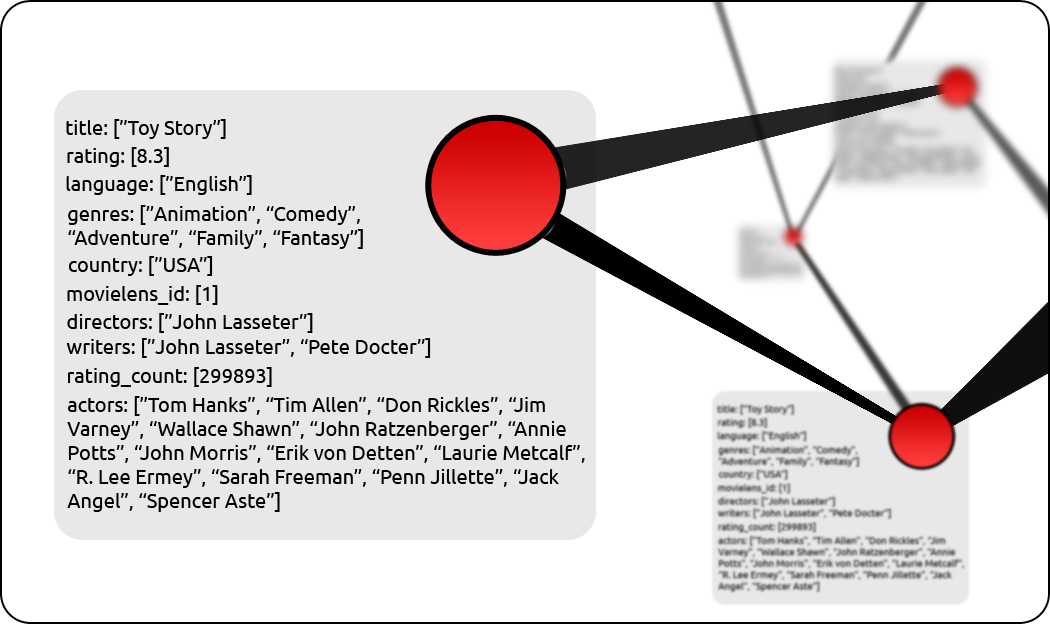
\includegraphics[scale=0.2]{Results/nodes.png}
\caption{Each item is represented by a node. The attributes of the item form the properties of the node.}
\label{node_G}
\end{figure}

\begin{figure}[htp]
\centering
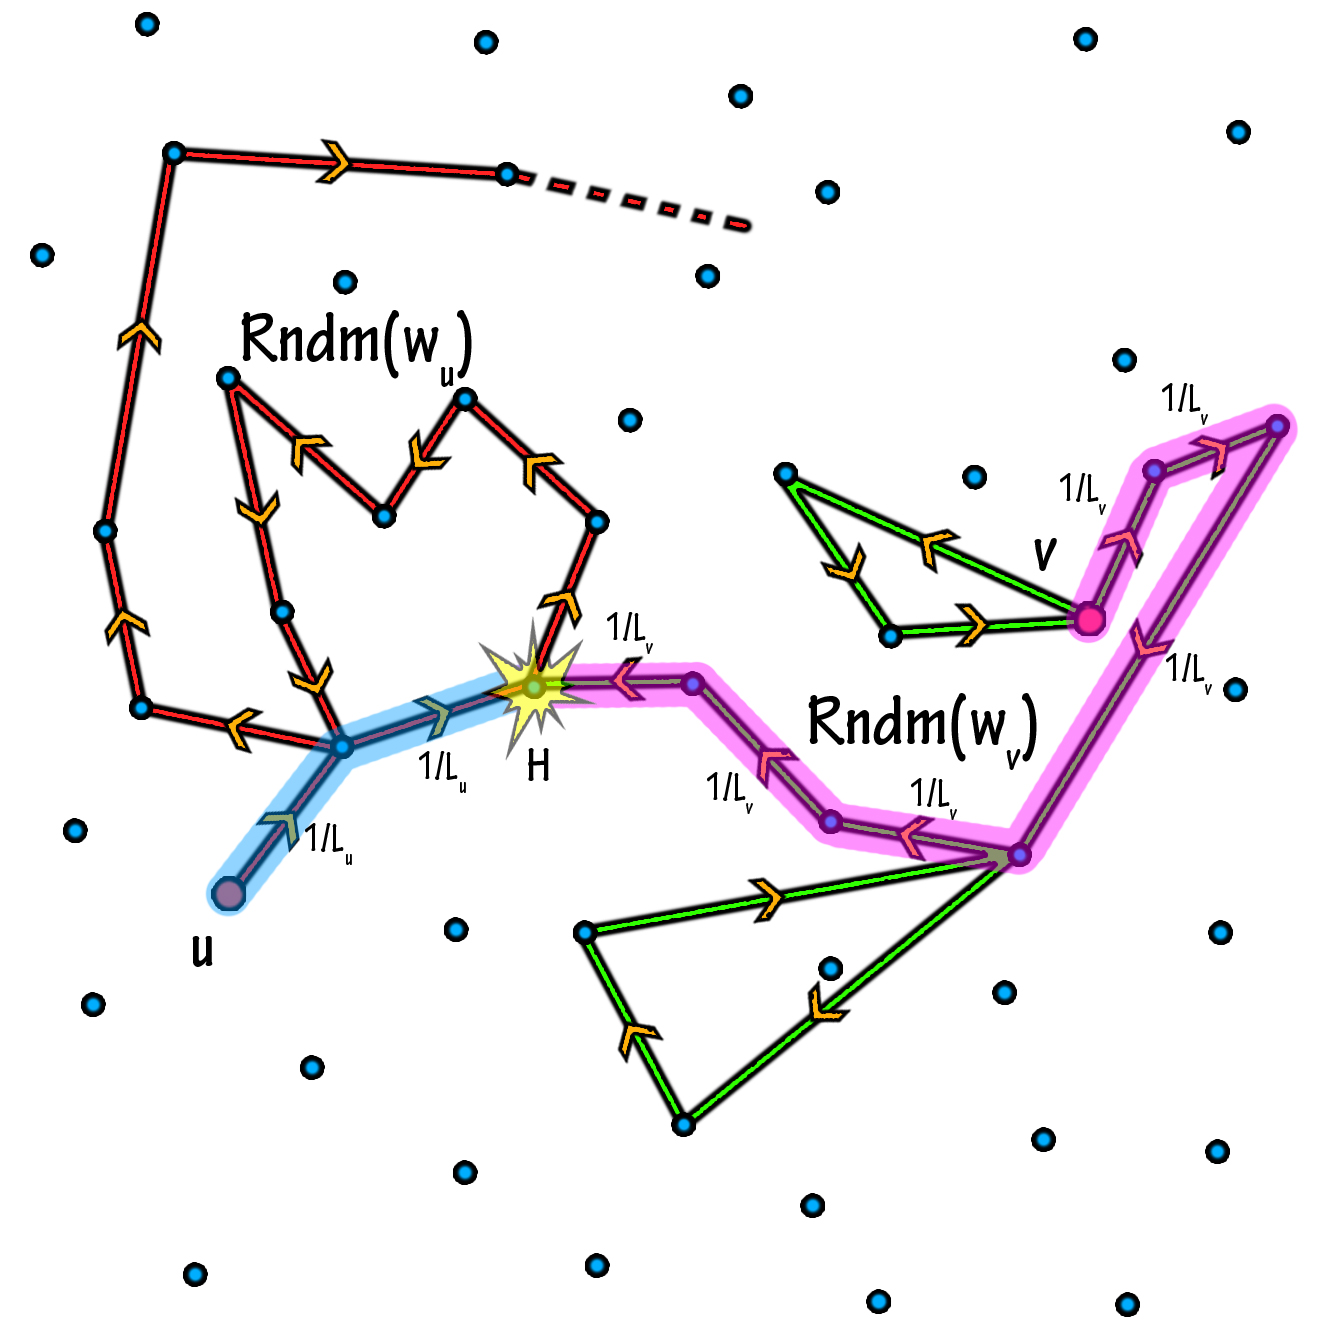
\includegraphics[scale=0.05]{Results/LearningComponent.jpg}
\caption{Items are connected to one another by edges. The attributes of the edges are the common attribute-value pairs between the end nodes.}
\label{edge_G}
\end{figure}

\begin{algorithm}
\label{keyValueNodesCategorical_algo}
\caption{Constructing $KeyValueNodes$ for categorical data}
\begin{algorithmic}[1]
    \STATE put the algorithm here
\end{algorithmic}
\end{algorithm}

\begin{algorithm}
\label{keyValueNodesNonCategorical_algo}
\caption{Constructing $KeyValueNodes$ for non-categorical data}
\begin{algorithmic}[1]
    \STATE put the algorithm here
\end{algorithmic}
\end{algorithm}

\subsection{Generating User Profiles}
\label{sec:userProf}
% ~\cite{stuart} search papers on user profiling\\

A user is an entity who consumes an item. In this section, we build a profile for each user. The user profile consists of characteristic features of the user that quantifies his behavior.

In real world, many factors influence the decision of the user to consume a particular item. These factors include the personal choices of the user and recommendation by other users. This scenario is analogous to a customer at a restaurant. The customer might place an order due to recommendations by his friends. His decision is also influenced by what he personally prefers to eat. Generally, the customer does not have equal preferences towards all properties of the food, such as sour, salt, hot and sweet. He has varied levels of liking towards various attributes. For a particular property, say sweet, the user may make choice based on the intensity of the flavor. Also, the customer might choose to place the order according to his preference or others' recommendation, with a certain weight. We generalize and quantify these behaviours of the customer in order to deduce the characteristic features of the customer.

It is easy to see that users behave in a similar manner, regardless of the type of item. We define two characteristic features associated with every user. In general, a user does not have equal preference towards all the attributes of the item. The preferences can be modeled as the weight that a user gives for each attribute of the item dataset. Further, the preferences of the user towards the values of a particular attribute is also modeled as weights. This forms the first characteristic feature $w_{u_p}$. While consuming an item, the user might decide upon the item purely based on his preferences or follow others' recommendations. We define $\alpha_{u_p}$ to be the probability with which the user $u_p$ decides upon an item purely based on his preferences. $\alpha_{u_p}$ quantifies how \emph{idiosyncratic} a user is. Closer the value of $\alpha_{u_p}$ to 1, more idiosyncratic the user is. The user follows others' recommendation with a probability $1-\alpha_{u_p}$. This forms the second characteristic 
feature.

$userProfile_{u_p} = \{w_{u_p}, \alpha_{u_p}\}$

In order to deduce the $w_{u_p}$ for a user $u_p \in U$, we construct an induced subgraph of the items that $u_p$ has rated. The properties of the edge capture the attribute-value pairs that are common between the end nodes. We hypothesize that, higher the importance that a user gives for an attribute and a value, higher the frequency of its existance as an edge property. Conversely, the frequency of occurance of attribute-value pair as a property of the edges is proportional to the importance that the user gives. In order to determine the relative importance of each attribute, we divide the corresponding frequency by the sum of frequencies. For a given attribute, we perform the same action to find out the relative importance of each value assumed by the attribute.

In the current setup, it is not possible to determine how idiosyncratic a user is. Such a behavior can only be determined when the system is able to receive feedback from the user. Hence, we set its value to $0.5$. Algorithm~\ref{userProf_algo} illustrates the methodology that we have developed to determine $w_{u_p}$ for a user $u_p \in U$.

%unsupervised learning???

\begin{algorithm}
\label{userProf_algo}
\caption{Creating User Profiles}
\begin{algorithmic}[1]
  \STATE put the algorithm here
\end{algorithmic}
\end{algorithm}

Figure~\ref{attribRelFreq_user} shows the relative importance of attributes for users $2987$, $3552$ and $5997$ from the MovieLens Dataset.

\begin{figure}[htp]
\centering
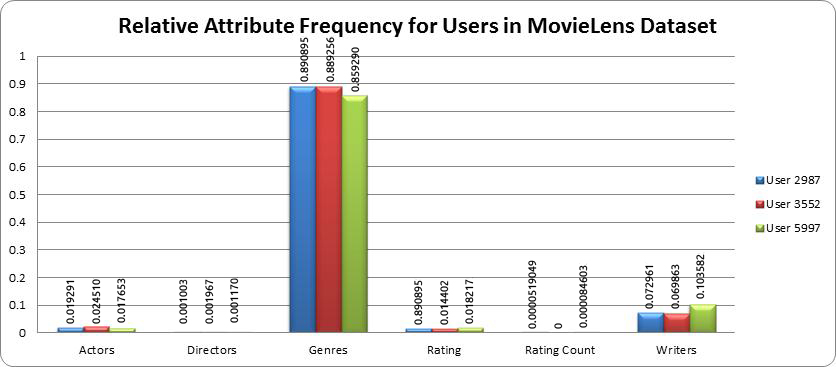
\includegraphics[scale=0.3]{Results/attribRelFreq_user.jpg}
\caption{The bar graph indicates the weights that users $2987$, $3552$ and $5997$ (from the MovieLens Dataset) have given to the corresponding attributes.}
\label{attribRelFreq_user}
\end{figure}

\subsection{Dimensionality Reduction for Items}
\label{sec:dimRed}
% ~\cite{badrul}, ~\cite{cureton}, ~\cite{deerwester}, ~\cite{berry}

Dimensionality Reduction is a well studied problem in recommender systems. Several methods, such as Latent Semantic Indexing~\cite{badrul} and Principal Component Analysis~\cite{cureton} etc, have been formulated to reduce the dimensions of the datasets. In this section, we present an empirical approach to perform dimensionality reduction on the dataset. We observe the users' pattern in consuming the items and deduce the importance of an attribute.

The importance of an attribute and its value in the item dataset increases as number of users who give higher relative importance to that attribute and its value increases. Hence, the importance of an attribute $a$ in the item set $I$ can be quantified as the mean relative importance of $a$, taken over all the users $u \in U$. Similarly, for an attribute $a$, the importance of a value $v$ is computed as the mean relative importance of $v$ for the attribute $a$, taken over all the users $u \in U$. In the previous section, we created a profile for each user. The characteristic feature $w_{u_p}$ consists of relative weights of attributes and its values for $u_p$. The relative importance of an attribute $a$ in the item set $I$ can be computed as follows:

$weight_a = \frac{\sum_{u_p \in U} w_{u_p}[a]}{Number\ of\ Users}$

Similarly, the relative importance of a value $v$ of attribute $a$ in the item set $I$ can be computed as follows:

$weight_{v_a} = \frac{\sum_{u_p \in U} w_{u_p}[a][v]}{Number\ of\ Users}$

Algorithms ~\ref{dimRedAttrib_algo} and ~\ref{dimRedValue_algo} illustrate the process of dimensionality reduction.

\begin{algorithm}
\label{dimRedAttrib_algo}
\caption{Dimensionality Reduction of Attributes}
\begin{algorithmic}[1]
  \STATE put the algorithm here
\end{algorithmic}
\end{algorithm}

\begin{algorithm}
\label{dimRedValue_algo}
\caption{Dimensionality Reduction of Values}
\begin{algorithmic}[1]
  \STATE put the algorithm here
\end{algorithmic}
\end{algorithm}

The dimensions of the dataset can then be reduced either by thresholding or selecting the top N dimensions with highest weights. Figure~\ref{attribRelFreq_items} shows the weights for various dimensions of the aggregated MovieLens Dataset.

\begin{figure}[htp]
\centering
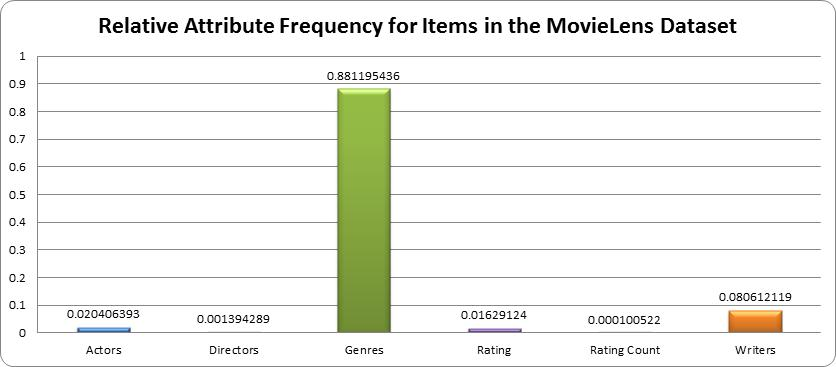
\includegraphics[scale=0.4]{Results/attribRelFreq_items.jpg}
\caption{The figure indicates the weights for various dimensions of the aggregated MovieLens Dataset, calculated using the above formula.}
\label{attribRelFreq_items}
\end{figure}

%unsupervised learning??

\subsection{Computing Similarity between Users}
\label{sec:userSimilarity}
% ~\cite{alexander}

The techniques involved in Collaborative Filtering are based on analyzing a large amount of data on users' activities and predicting what the a given user might like. The recommendations can be based on similarity between users or similarity between items. Our algorithm uses similarity between users to perform collaborative filtering. Some of the popular similarity measures are Euclidean Distance, Cosine Similarity, Pearson Correlation and Jaccard Similarity. ~\cite{alexander} presents a comparative study of the impact of these similarity measures on web page clustering.

Jaccard similarity is a measure used for comparing the similarity of sample sets. Jaccard similarity between two sets $A$ and $B$ is mathematically defined as follows:\\
$J(A,B) = \frac{|A \cap B|}{|A \cup B|}$\\
Each user is associated with a set of items that he has consumed. The similarity between users can be computed just by applying the simple Jaccard similarity between the sets of items for a pair of users. But there is an intrinsic drawback associated with this approach. The approach treats all the items to be equivalent. It is ignorant towards the properties of the items themselves and the relations between them. To include these considerations, we modify the simple formula for Jaccard similarity.

The idea behind the modification is as follows. To compute the similarity between two users $u_p$ and $u_q$, we compute two induced subgraphs of $G$. One of them contains the intersecting items of the two users, and the other contains the union of items of the two users. From the two induced subgraphs, we make two aggregated lists of edge attributes, one for each subgraph. Note that the attributes in these lists can repeat. The similarity is calculated as a fraction. To compute the numerator, we iterate  through the attributes in the aggregated list for item intersection subgraph. Counting the number of occurances of these attributes would implicitly mean that we are considering all the attribute as equals. But, the users give varied levels of importance to the attributes. Hence, for each attribute in the aggregated list, we sum up the corresponding weights from the users $u_p$ and $u_q$ and multiply the sum by the relative frequency of occurance of the attribute in the aggregated list. We follow a similar 
procedure to compute the denominator, with the only difference being that we consider the item union subgraph.

$Intrscn = [a\ |\ a \in edge\ attribute\ of\ subgraph(items\ of\ u_p\ \cap items\ of\ u_q, G)]$\\
\newline
$Union = [a\ |\ a \in edge\ attribute\ of\ subgraph(items\ of\ u_p\ \cup items\ of\ u_q, G)]$\\
\newline
$sim(u_p, u_q) = \frac{\sum (w_{u_p}[a]\ +\ w_{u_q}[a])*relFreq(a, Intrscn)\ \forall\ a\ \in\ set(Intrscn))}{\sum (w_{u_p}[a]\ +\ w_{u_q}[a])*relFreq(a, Union) \forall\ a\ \in\ set(Union))}$

where $relFreq(attrib, list)$ returns the relative frequency of occurance of $attrib$ in $list$.

Algorithm~\ref{userSimilarity_algo} illustrates the computation of similarity between all pairs of users $(u_p, u_q) \in U$. Note that $U_{sim}$ is symmetric in nature. Hence, the amount computation can be reduced approximately by half to make the implementation more efficient.

\begin{algorithm}
\label{userSimilarity_algo}
\caption{Computing User Similarity}
\begin{algorithmic}[1]
  \STATE Put the algorithm here
\end{algorithmic}
\end{algorithm}

\subsection{Clustering the Users}
\label{sec:clustering}
The previous section dealt with computing the similarity between the users. The similarities thus computed are then used to cluster the users into various groups. In our approach, we are performing overlapping clustering, wherein each user may belong to more than one cluster. Clustering the users in this manner is important because more similar a pair of users are, higher their impact on each other's recommendations. The clustering mechanism we use is as follows. If two users have similarity scores greater than a threshold, then the two users belong to the same cluster. The number of clusters formed depends on the distribution of the similarity scores across all the pairs of users. The threshold is set as the average similarity score across all the users. Algorithm~\ref{clustering_algo} depicts the approach explained above.

\begin{algorithm}
\label{clustering_algo}
\caption{Clustering users}
\begin{algorithmic}[1]
  \STATE Put the algorithm here
\end{algorithmic}
\end{algorithm}

\section{Recommendation Algorithm}
In section~\ref{sec:preparation}, we created a set of reference structures that will aid us in recommending items to users. In the subsequent sections, we will use these reference structures to recommend new items to users. We present two approaches of recommending items to users. The Idiosyncratic approach considers only the history of the user in order to recommend new items. The Collaborative Filtering approach considers the clusters to which the user belongs and the user's similarity with the other users in the cluster to provide recommendation. The recommendations from both the approaches are then combined to produce a hybrid recommendation.

\subsection{Idiosyncratic Recommendation}
\label{sec:idiosyncratic}
% Egocentric Recommendation considers only the history of the user in order to recommend new items to the user. It does not take into consideration the relationship of the user with other users.

The idiosyncratic algorithm works as follows. We initialize the scores of all the items to zero. Given a user $u$, we analyze the list of items that $u$ has previously consumed. For each item that has not been consumed by $u$, we capture a set of weights and ratings. A weighted average of these ratings will yield the predicted ratings for the item under consideration. The weights and ratings are considered for each attribute-value pair. The weight is computed as a function of the user's weights for the attribute-value pair. The rating is computed as the average rating given by the user for the items possessing the corresponding attribute-value pair. The items are then sorted in the decreasing order of their predicted ratings to get the recommendation list. Algorithm~\ref{idiosyncratic_algo} explains the approach in detail.

\begin{algorithm}
\label{idiosyncratic_algo}
\caption{Idiosyncratic Rating Prediction}
\begin{algorithmic}[1]
  \STATE Put the algorithm here
\end{algorithmic}
\end{algorithm}

% On sorting $scores\_ego$ in the decreasing order, we get a pure egocentric recommendation list. In the next subsection, we describe the methodology to obtain a similar list using Collaborative Filtering techniques. It is possible to combine the obtained list with $scores\_ego$ to get a hybrid recommendation. We describe two methods of combining the lists in section~\ref{sec:hybrid}.

\subsection{Collaborative Filtering based on User Similarity}
\label{sec:collab}
Collaborative Filtering(CF) is a collection of techniques that are used in recommending items to users based on the ratings of other users. CF techniques are one of the most successful techniques in recommending items to users. The core idea behind CF techniques is the concept of similarity. The recommender systems generally use two forms of similarities: user-based similarities and item-based similarities. These techniques generally use a standard metric, such as Euclidean Distance, Cosine Similarity, Pearson Correlation or Jaccard Similarity. Once a similarity matrix is built, these systems use various algorithms to generate recommendations.

In this paper, we have used an extended version of Jaccard similarity, as described in section~\ref{sec:userSimilarity}. The algorithm that we have developed uses user-based similarity. The predicted ratings of items for the user $u$ is computed in the following way. The algorithm begins by iterating through all the clusters that $u$ is a part of. A cluster houses many users. Each user is associated with a list of items that he has consumed. For every other user $u_p$ in each of those clusters $c$, we analyze the list of items consumed by $u_p$. For each item, the rating given by $u_p$ and the similarity between $u$ and $u_p$ is noted. For a given item, it is clear that the rating and corresponding similarities get accumulated as the algorithm proceeds. To predict the rating for an item, a weighted average of the ratings is computed, with the similarities as the weight.

Note that the clusters we obtained are overlapping. That is, a single user can belong to multiple clusters. If the given user $u_1$ is very similar to another user $u_2$, then $u_2$ will appear in majority of the clusters where $u_1$ is present. This implies that the score for the items consumed by $u_2$ is naturally boosted, since $u_2$ is presented in most of $u_1$'s clusters and the similarity between $u_1$ and $u_2$ is high. Algorithm~\ref{collab_algo} depicts the approach explained above.

\begin{algorithm}
\label{collab_algo}
\caption{Collaborative Recommendation based in User Similarity}
\begin{algorithmic}[1]
  \STATE put the algorithm here
\end{algorithmic}
\end{algorithm}

Algorithms~\ref{idiosyncratic_algo} and ~\ref{collab_algo} generated $recommendedItemsIdio$ and $recommendedItemsColl$, a pure idiosyncratic recommendation list and a pure collaborative recommendation list respectively. In the next subsection, we describe a method to combine these two lists to get a hybrid recommendation.

\subsection{Hybrid Recommendation}
\label{sec:hybrid}
Sections~\ref{sec:idiosyncratic} and~\ref{sec:collab} dealt with generating idiosyncratic and collaborative recommendations for the user. Both the algorithms associated a rating with each item that a user has not consumed. Hybrid Recommendation involves combining these two lists into a single list $recommendedItemHybrid$, by means of a weighted combination of ratings or ranks of corresponding items from both the lists.

Since we are merging the lists that signify idiosyncratic behavior and group behavior, we choose $\alpha_{u_p}$ as the weight. In section~\ref{sec:userProf}, we had defined $\alpha_{u_p}$ as the probability with which the user $u_p$ decides upon an item purely based on his preferences. $\alpha_{u_p}$ quantifies how \emph{idiosyncratic} a user is. Hence, we assign a weight $\alpha_{u_p}$ to $recommendedItemsIdio$ and $1 - \alpha_{u_p}$ to $recommendedItemsColl$.

We propose two methods by which the lists can be combined:
\begin{enumerate}
 \item Rank based weighted average:\\
 In this approach, we take a weighted average of ranks of each item and sort the items in the decreasing order of their composite ranks. The following formula mathematically describes the operation:\\
 $compositeRank_i = \alpha_{u_p}*rank(i, recommendedItemsIdio) + (1 - \alpha_{u_p})*rank(i, recommendedItemsColl)$
 
 \item Score based weighted average:\\
 In this approach, we take a weighted average of score of each item and sort the items in the decreasing order of their composite scores. The following formula mathematically describes the operation:\\
 $compositeScore_i = \alpha_{u_p}*recommendedItemsIdio[i] + (1 - \alpha_{u_p})*recommendedItemsColl[i]$
\end{enumerate}

Rank based weighted average method can be used to provide recommendations to the user in the order of their ranks. But, evaluating the accuracy of our algorithm also tends to be relatively hard since our system assumes the absence of feedback. Hence, in our experiments, we use the score based weighted average method to predict the rating that a user might give to an unseen item.

%As an alternative approach, we could let the user set the value of alpha.

\section{Results and Discussions}
\label{sec:results}
\subsection{Dataset}
As mentioned in section~\ref{sec:dataset}, we have used the aggregated MovieLens Dataset in our experiments. We have used the dataset with 1 Million ratings from 6000 users on 4000 movies, and retrieved the metadata about the movies from\\
\emph{http://imdbapi.org/} and \emph{http://www.omdbapi.com/}. We split the user dataset into two parts, training data and test data. The training data constitutes 70 percent of the dataset. The users in the training set were chosen randomly. We test the accuracy of our algorithm by predicting the user ratings in the remaining 30 percent of the dataset.

\subsection{Evaluation Metric}
% Evaluation of Recommender Systems, Resnik et al 1994
% Evaluating Collaborative Recommender Systems, Jonathan L. Herlocker
% Evaluating Recommendation Systems, G Shani, A Gunawardhana, Recommender Systems Handbook, 2011, Springer

The performance of recommender systems have been extensively studied in research literature since 1994~\cite{resnick}.~\cite{jonathan} broadly classifies recommendation accuracy metrics into three classes: predictive accuracy metrics, classification accuracy metrics and rank accuracy metrics. In this paper, we have chosen to evaluate our algorithm using a type of predictive accuracy measure called \emph{Root Mean Square Error} (RMSE). Root Mean Square Error is a common metric that is used to evaluate the accuracy of prediction algorithms. It is defined as the square root of average of error squares, with the error being taken as the deviation of the predicted rating from the actual rating. The mathematical definition of RMSE is as follows:

$RMSE = \sqrt{\frac{1}{|S_{test}|} \sum_{(u,i) \in S_{test}} (R_{ui} - T_{ui})^2}$

\subsection{Experimental Results}
In this section, we present the results obtained on applying our algorithm to the aggregated MovieLens Dataset. Section~\ref{sec:buidingItemGraph} dealt with the creation of item graph $G$. Given two movies from the dataset, just a single common attribute-value pair will result in an edge formation. For example, if two movies are of the same language, an edge is formed between them. Hence, the graph that we obtain is fairly dense. After transforming the aggregated MovieLens dataset, we found that $G$ was a very dense graph, with a density of <insert density here>, with an average degree of <insert degree here>.

% Figures~\ref{node_G} and~\ref{edge_G} show a more elaborate view of the structure of $G$.
% 
% \begin{figure}[htp]
% \centering
% 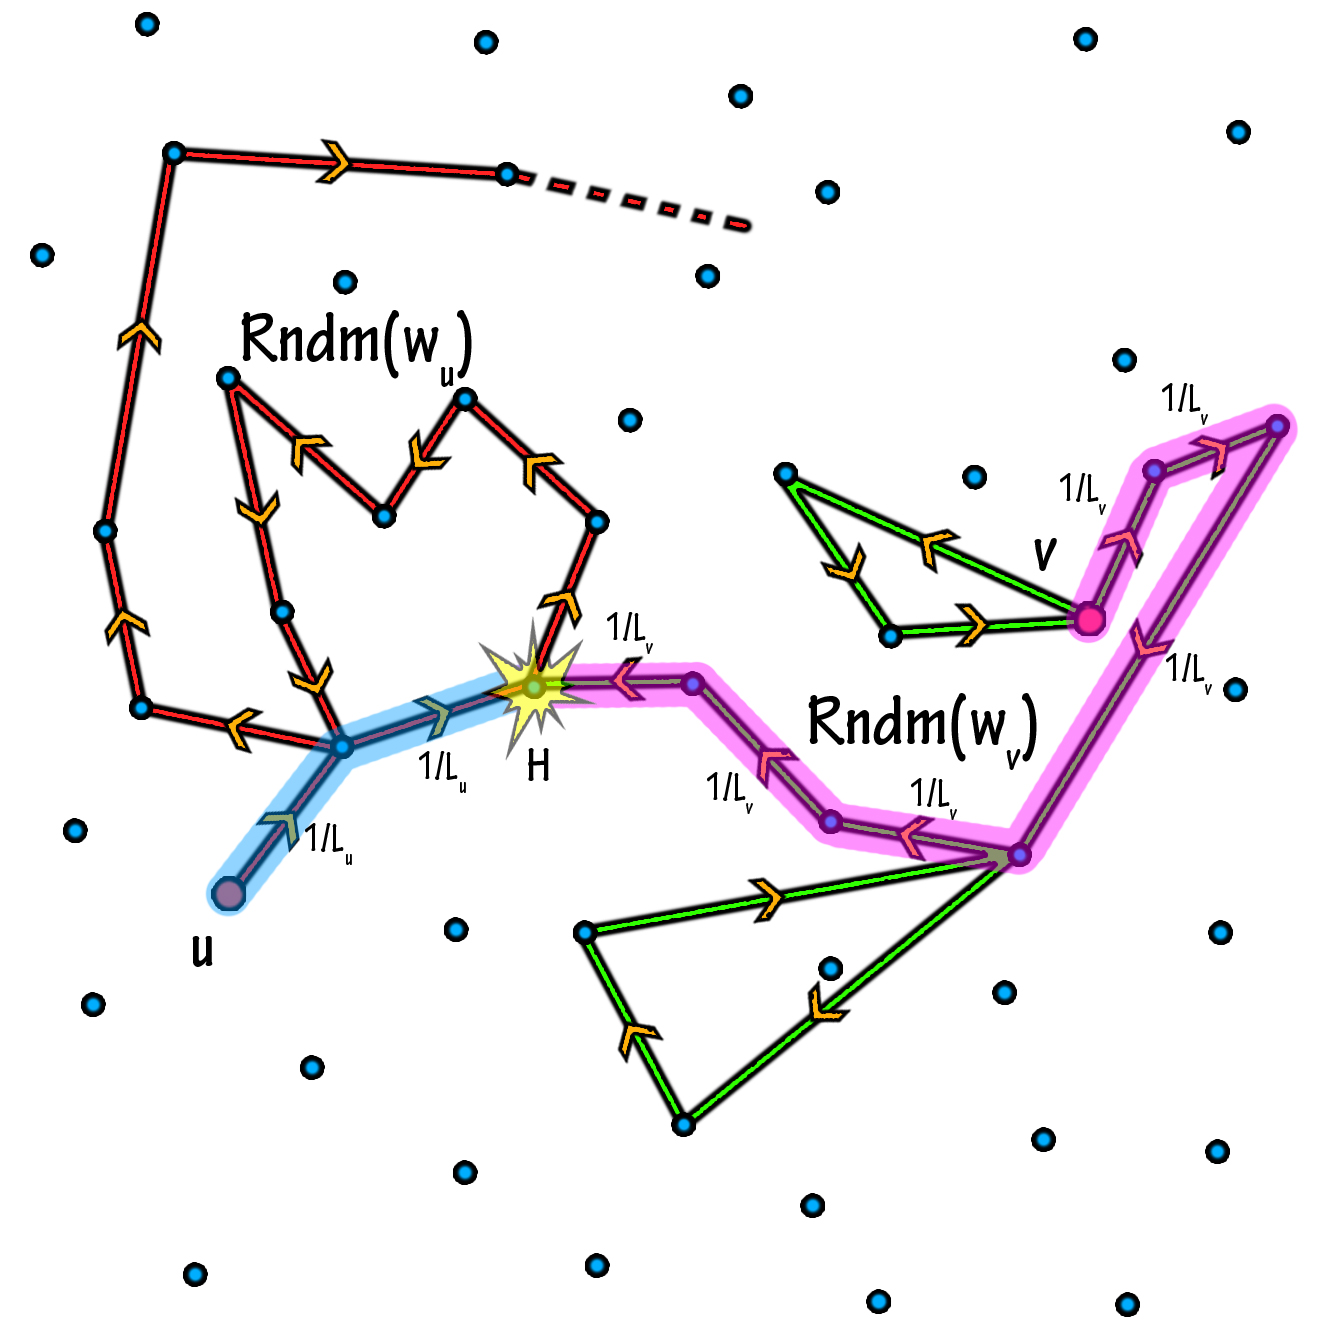
\includegraphics[scale=0.05]{Results/LearningComponent.jpg}
% \caption{Snapshot of $G$. The graph is built using the aggregated MovieLens dataset}
% \label{movielens_itemGraph}
% \end{figure}

In section~\ref{sec:userProf}, we created the profiles for each user, $userProfile_{u_p}$. We also defined two characteristic features, $w_{u_p}$ and $\alpha_{u_p}$, for each user. We provided a methodology to determine $w_{u_p}$ in Algorithm~\ref{userProf_algo}.

Figure~\ref{movielens_attrRelFreq_user} statistically illustrates the weights for a randomly sampled user $2987$ of the MovieLens dataset, for various attributes. <insert analysis for the bar plot here. see the commented line below for guidance.>
% In general, it is very likely that the users watch the movies from the same country that they reside in. As far as the dynamics of shooting movies go, the filming locations of a movie are likely to be in the same country that the movie is being produced. In general, users who are familiar with a particular language tend to watch the movies from the same language. Naturally, the weights for country, filming locations and language are relatively high. The fact that there are comparitively limited number of values for a particular also boosts up the relative score. The ratio between relative scores indicates the number of times that a particular attribute is important, relative to the other. From the figure, we can deduce that the user $2987$ statistically gives $37.3$ times more importance to actors, compared to directors. On similar lines, user $2987$ gives 3.5 times more importance to genre, compared to actors.

\begin{figure}[htp]
\centering
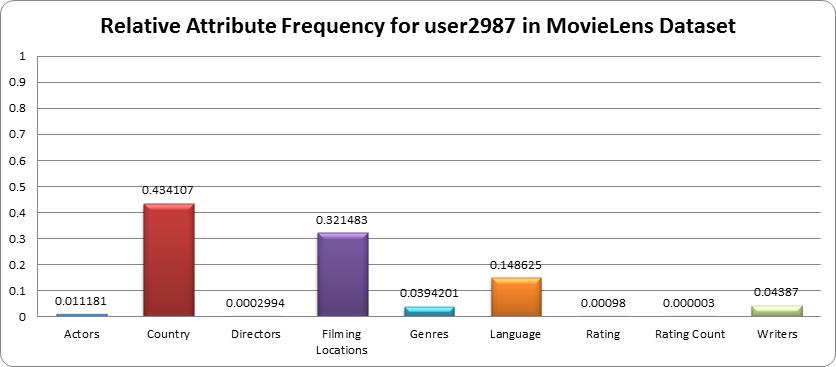
\includegraphics[scale=0.38]{Results/movielens_attrRelFreq_user2987.jpg}
\caption{Relative Attribute Importance for a randomly sampled user $2987$ of the MovieLens dataset}
\label{movielens_attrRelFreq_user}
\end{figure}

Figure~\ref{movielens_valRelFreq_user} illustrates the relative value importance for the attribute <insert attrib here>.

\begin{figure}[htp]
\centering
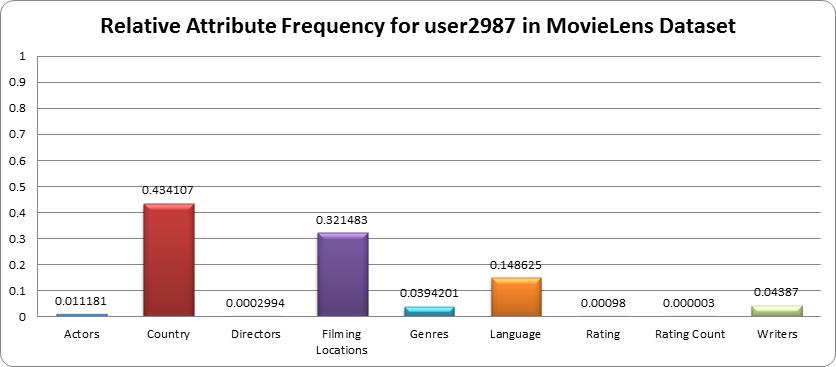
\includegraphics[scale=0.38]{Results/movielens_attrRelFreq_user2987.jpg}
\caption{Relative Value Importance for the attribute <insert attrib here>, for a randomly sampled user $2987$ of the MovieLens dataset}
\label{movielens_valRelFreq_user}
\end{figure}

In section~\ref{sec:dimRed}, we reduced the dimensionality of the dataset based on the relative importances that each user gives to a particular attribute. We apply the same techinique to the aggregated MovieLens dataset. Figure~\ref{movielens_attrRelFreq_item} shows the relative attribute importance for the dataset.

\begin{figure}[htp]
\centering
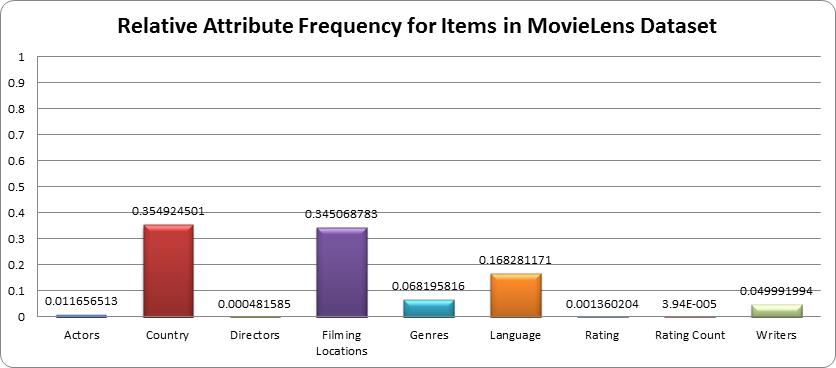
\includegraphics[scale=0.38]{Results/movielens_attrRelFreq_item.jpg}
\caption{Relative Attribute Importance of the items in the MovieLens dataset}
\label{movielens_attrRelFreq_item}
\end{figure}

We analyze the data for the entire aggregated MovieLens dataset in the same way as we did for user $2987$. On an average, we find that the users statistically give <insert ratio here> times more importance to actors in comparison with directors. On similar lines, users give <insert ratio here> times more importance to genres, compared to actors.

% In section~\ref{sec:userSimilarity}, we modified the simple Jaccard similarity to include information about the items and user preferences as well. In section~\ref{sec:clustering}, we classified the users into overlapping clusters.

% <visualization of cluster??? yes if possible>

To evaluate the accuracy of our algorithm, we use RMSE as the evaluation metric. We use $\alpha_{u_p}$ as a parameter in our experiments. Zhouxiao Bao and Haiying Xia, in their paper titled "Movie Rating Estimation and Recommendation", build a movie rating prediction system based on the training sets provided by MovieLens. The paper was written as a part of their final project in Machine Learning course, Autumn 2012 at Stanford University. They present various approaches that signify the Root Mean Square Error on changing the parameters for various predictor algorithms. We use the results obtained by their works as a benchmark on comparison to our algorithm. Bao and Xia, in their paper, have chosen MovieLens 100k Dataset as the training set. This dataset contains 100,000 ratings from 943 on 1682 movies, in which each user has rated at least 20 movies. Among MovieLens 100k Data Set, they choose ua.base/test and ub.base/test for result comparison between different training sets and testing sets. The whole set 
u data is split into a training set and a test set with exactly 10 ratings per user in the test set. The sets ua.test and ub.test are disjoint.
\begin{center}
  \begin{tabular}{| c | c |}
    \hline
    Algorithms & RMSE \\ 
    & or argmin RMSE \\ \hline \hline
    Baseline Predictor on ub dataset & 0.97737 \\ \hline
    Baseline Predictor on ua dataset & 0.96648 \\ \hline
    K-Nearest Neighbor & 0.95* \\ \hline
    Stochastic Gradient & 0.943* \\ \hline
    SVD & 0.939* \\ \hline
    SVD ++ & 0.926* \\ \hline
    Asymmetric SVD & 0.924* \\ \hline
    Global Neighborhood & 0.931926 \\ \hline
    Co-clustering BVD & 0.917* \\ \hline
    Approach discussed in this paper & 0.9031 \\ \hline
  \end{tabular}
\end{center}

* argmin RMSE

As seen from the table above, the approach discussed in this paper produces a smaller error in predicting ratings of a larger dataset, but at the cost of using item-related data. Note that majority of the approaches mentioned here are parameterized. i.e, the algorithm must be re-run by varying certain parameters to find a point, the minima, at which the performance is optimized.

% For varying values of $\alpha_{u_p}$, we predict each user's ratings for all the movies that the user has not rated in the training set. We compare these predicted ratings with the actual ratings present in the test set and compute the MAE. The variation of MAE for various values of $\alpha_{u_p}$ is shown in Figure~\ref{movielens_mae_alpha}.

% \begin{figure}[htp]
% \centering
% 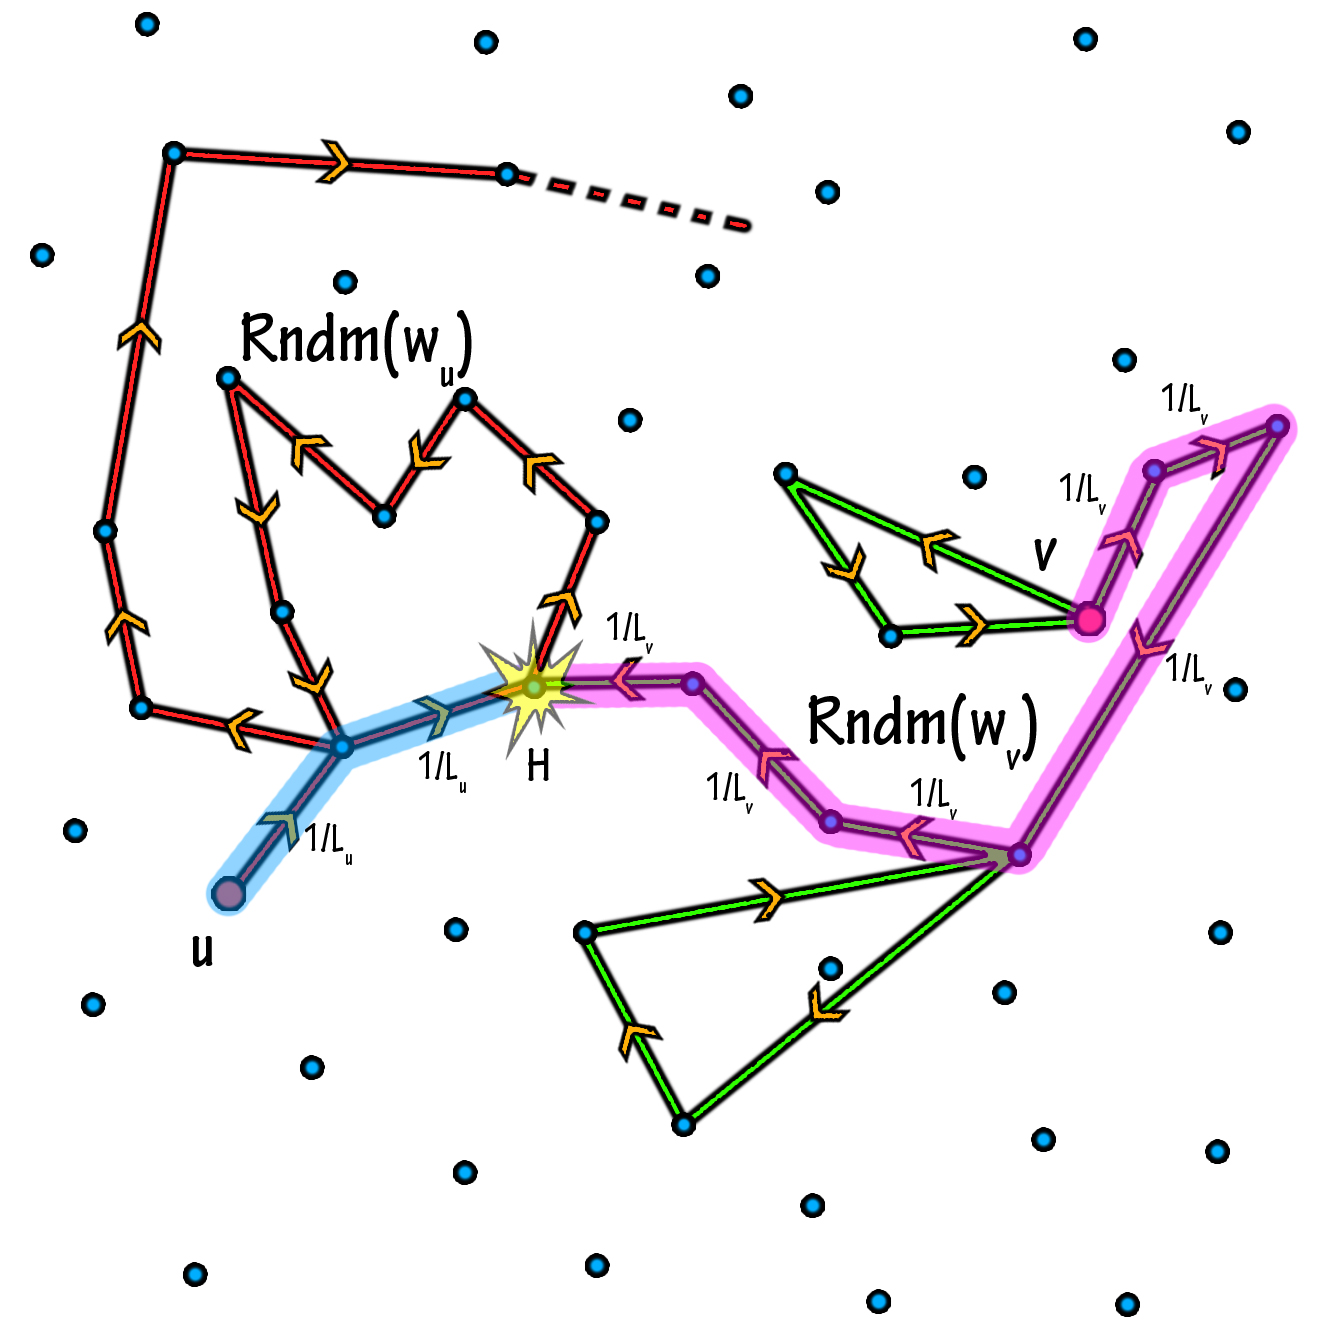
\includegraphics[scale=0.05]{Results/LearningComponent.jpg}
% \caption{The plot of variation of Mean Absolute Error with varying values of $\alpha_{u_p}$}
% \label{movielens_mae_alpha}
% \end{figure}

% Explain what happens at extreme points, i.e, at $\alpha_{u_p} = 0$ and $\alpha_{u_p} = 1$

% refer to the dataset explanation
% refer to figure with nodes and edges - for building graph
% sample diagram with weights for attributes for multiple users
% 
% describes our experimental work
% details of our dataset, evaluation metrics, methodology, results of different experiments and discussions.

\section{Conclusion}
\label{sec:conclusion}
In this paper, we demonstrated a novel approach for recommending items to users and performed experiments on the aggregated MovieLens dataset to test our algorithm. We use graph as the core reference structure. We form a graph of items and the relations between items are manifested as properties of the corresponding edges. Based on the users' history of item consumption, we profile each user and deduce the weight that the user gives to the attributes and their corresponding values. We use the profiles to statistically determine the importance of each attribute in the dataset, in turn performing dimensionality reduction on the item dataset. To find out the similarity between users, we modified the simple Jaccard similarity to consider the properties of users and items. Based on a similarity threshold, we form overlapping clusters of users. To provide recommendation for a particular user, we follow two distinct approaches: idiosyncratic and collaborative filtering. These recommendations are then combined to 
form a hybrid recommendation.

We test our approach on the aggregated Movielens dataset. Our results show that the importance of each dimension of the dataset can be computed in accordance with the pattern that the users follow to consume the items. We deduce and depict the relative importance that each user gives to each of the attributes and their corresponding values. Using this data, we also perform dimensionality reduction on the Movielens dataset and plot the relative weights. The recommendations that we provide to a user is personalized based on the corresponding relative importances of the user. We then compare the accuracy of our approach with other parameterized and non-parameterized approaches such as KNN, SVD, BVD etc. It is found that the approach discussed in this paper produces a smaller error in predicting the ratings of a larger dataset, but at the cost of using item-related data.

\section{Future Work}
The idea behind the approach can be extended to function as a link prediction algorithm for a social network. A recommendation problem can be manifested as a link prediction problem if the item dataset and the user dataset are the same. If the user dataset of a social network is appropriately mapped to the inputs to our approach, it is possible to predict the forthcoming links in the network.

The approaches for user profiling and dimensionality reduction on the item dataset have a lot of scope for improvement and quality measurement, when experimented on a various other datasets.

Our experiments were performed on the MovieLens dataset of an intermediate size, with a restricted number of ratings and users. The tests must be performed on larger datasets, with a wide variety of attributes. The characteristic feature $\alpha_{u_p}$ represents how idiosyncratic a user is. Determining the value of this parameter demands for a feedback mechanism from the users.

In this paper, we have presented the empirical results that we have obtained on applying our algorithm on the dataset. The theoritical bounds of the algorithm is yet to be formulated. The approach presented in this paper does not enforce all the items to have the same set of attributes, i.e, the attributes need not be homogeneous across all the items. In our experiments, we have chosen a homogeneous dataset. The tests must be performed on heterogeneous datasets, where it is not necessary that all items have the same set of attributes.

\section{Acknowledgements}
The work was conducted at PES Institute of Technology, West Campus, Bengaluru, India. We would like to thank Prof. Nitin V Pujari, HOD, Department of Computer Science, PESIT and Dr. KNB Murthy, Principal, PESIT for providing us with an opportunity to carry out the research work. We also thank anonymous reviewers for their valuable comments.
\newpage
\bibliographystyle{plain}
\bibliography{references}

\end{document}